\documentclass[11pt, a4paper]{article}
\usepackage[utf8]{inputenc}
\usepackage[margin=1in]{geometry} %Sets proper 1-inch margins. 
\usepackage{amsmath} %Only load this if you are using math/equations.
\usepackage{graphicx} %Only need to call this if inserting images.
\usepackage{caption} %Only need to call this if inserting captions.
\usepackage{float} %Allows the use of the [H] specifier. 
\graphicspath{{C:/Users/jonah/Pictures/meme/}} %Sets the working directory for images.
\usepackage[colorlinks,citecolor=blue,linkcolor=blue,urlcolor=blue]{hyperref} %Allows for the embedding of urls. 
\usepackage{setspace}
\usepackage{blindtext}

\pagenumbering{arabic}

\usepackage{fancyhdr}

\pagestyle{fancy}
\fancyhf{}
\rhead{Jonah Edmundson \\ 2023}
\lhead{\thepage}

\newcommand{\comment}[1]{}

\usepackage{Sweave}
\begin{document}
\Sconcordance{concordance:variableinvestigation.tex:variableinvestigation.Rnw:%
1 23 1 1 0 19 1 1 2 1 0 3 1 1 6 5 0 1 3 1 0 1 3 1 0 1 12 14 0 1 2 8 1 1 %
3 2 0 1 2 1 0 1 2 1 0 1 2 6 0 1 6 9 0 1 2 3 1 1 4 3 0 1 2 8 0 1 7 9 0 1 %
2 6 1 1 2 1 0 1 7 9 0 1 2 1 5 10 0 1 8 11 0 1 2 2 1 1 14 17 0 1 2 30 1}


\begin{center}
\Large{\textsc{Variable Investigation}}
\par
\normalsize{\textsc{for}}
\par
\large{\textsc{Kelowna Weather-Crash Project}}
\end{center}


\vspace{0.917 pc} %Creates a paragraph line break. 

\tableofcontents


\pagebreak
%\section{Loading data}



\section{Summary Statistics}

\begin{Schunk}
\begin{Soutput}
Need to remove dew point temp and wind chill, 
since they are so correlated with temperature.
\end{Soutput}
\begin{Soutput}
                    Temp...C. Dew.Point.Temp...C. Wind.Chill
Temp...C.           1.0000000           0.9209662  0.9517406
Dew.Point.Temp...C. 0.9209662           1.0000000  0.9312014
Wind.Chill          0.9517406           0.9312014  1.0000000
\end{Soutput}
\begin{Soutput}
Summary of all variables:
\end{Soutput}
\begin{Soutput}
    linker          Date.Of.Loss.Year Animal.Flag              Crash.Severity 
 Length:56136       Min.   :2017      No :54118   CASUALTY CRASH      :11473  
 Class :character   1st Qu.:2018      Yes: 2018   PROPERTY DAMAGE ONLY:44663  
 Mode  :character   Median :2019                                              
                    Mean   :2019                                              
                    3rd Qu.:2020                                              
                    Max.   :2021                                              
                                                                              
 Cyclist.Flag    Day.Of.Week                Derived.Crash.Configuration
 No :55725    FRIDAY   :9316   REAR END                   :13024       
 Yes:  411    MONDAY   :8024   SINGLE VEHICLE             :12495       
              SATURDAY :6753   UNDETERMINED               :11453       
              SUNDAY   :5464   SIDE IMPACT                :11369       
              THURSDAY :9061   CONFLICTED                 : 3068       
              TUESDAY  :8728   SIDE SWIPE - SAME DIRECTION: 1833       
              WEDNESDAY:8790   (Other)                    : 2894       
 Heavy.Veh.Flag Intersection.Crash  Month.Of.Year   Motorcycle.Flag
 No :54085      No :31677          JULY    : 5152   No :55673      
 Yes: 2051      Yes:24459          DECEMBER: 5095   Yes:  463      
                                   JANUARY : 5063                  
                                   AUGUST  : 4907                  
                                   OCTOBER : 4836                  
                                   JUNE    : 4735                  
                                   (Other) :26348                  
 Parked.Vehicle.Flag Parking.Lot.Flag Pedestrian.Flag     Time.Category  
 No :38567           No :37189        No :55790       12:00-14:59:14870  
 Yes:17569           Yes:18947        Yes:  346       15:00-17:59:14473  
                                                      09:00-11:59:11021  
                                                      18:00-20:59: 5805  
                                                      06:00-08:59: 5489  
                                                      21:00-23:59: 2684  
                                                      (Other)    : 1794  
    Municipality.Name Road.Location.Description       Street.Full.Name
 KELOWNA     :45943   UNKNOWN     : 2211        HWY 97        : 6019  
 WEST KELOWNA:10193   HWY 97      : 1961        HARVEY AVE    : 3168  
                      HARVEY AVE  : 1670        HWY 33        : 2064  
                      LAKESHORE RD:  932        GORDON DR     : 1921  
                      LOUIE DR    :  751        LAKESHORE RD  : 1372  
                      HWY 33      :  715        SPRINGFIELD RD: 1326  
                      (Other)     :47896        (Other)       :40266  
 Total.Crashes   Total.Victims      Temp...C.       Rel.Hum....    
 Min.   :1.000   Min.   :0.0000   Min.   :-22.43   Min.   : 12.67  
 1st Qu.:1.000   1st Qu.:0.0000   1st Qu.:  1.60   1st Qu.: 38.00  
 Median :1.000   Median :0.0000   Median : 10.37   Median : 62.00  
 Mean   :1.006   Mean   :0.2917   Mean   : 10.92   Mean   : 60.51  
 3rd Qu.:1.000   3rd Qu.:0.0000   3rd Qu.: 20.00   3rd Qu.: 82.33  
 Max.   :3.000   Max.   :9.0000   Max.   : 37.73   Max.   :100.00  
                                  NA's   :35       NA's   :35      
 Precip..Amount..mm. Wind.Dir..10s.deg. Wind.Spd..km.h.  Visibility..km.
 Min.   :0.00000     Min.   : 1.00      Min.   : 0.000   Min.   : 0.20  
 1st Qu.:0.00000     1st Qu.:15.67      1st Qu.: 4.667   1st Qu.:16.10  
 Median :0.00000     Median :19.50      Median : 8.000   Median :16.10  
 Mean   :0.03111     Mean   :21.16      Mean   :10.277   Mean   :15.15  
 3rd Qu.:0.00000     3rd Qu.:31.00      3rd Qu.:13.667   3rd Qu.:16.10  
 Max.   :4.00000     Max.   :36.00      Max.   :51.333   Max.   :16.10  
 NA's   :35          NA's   :4020       NA's   :35       NA's   :36     
 Stn.Press..kPa. Fog       Freezing.Rain Snow      Rain      Thunderstorms
 Min.   :94.08   0:52106   0:56134       0:52325   0:50075   0:56002      
 1st Qu.:96.10   1: 4030   1:    2       1: 3811   1: 6061   1:  134      
 Median :96.51                                                            
 Mean   :96.56                                                            
 3rd Qu.:96.90                                                            
 Max.   :99.33                                                            
 NA's   :35                                                               
\end{Soutput}
\end{Schunk}
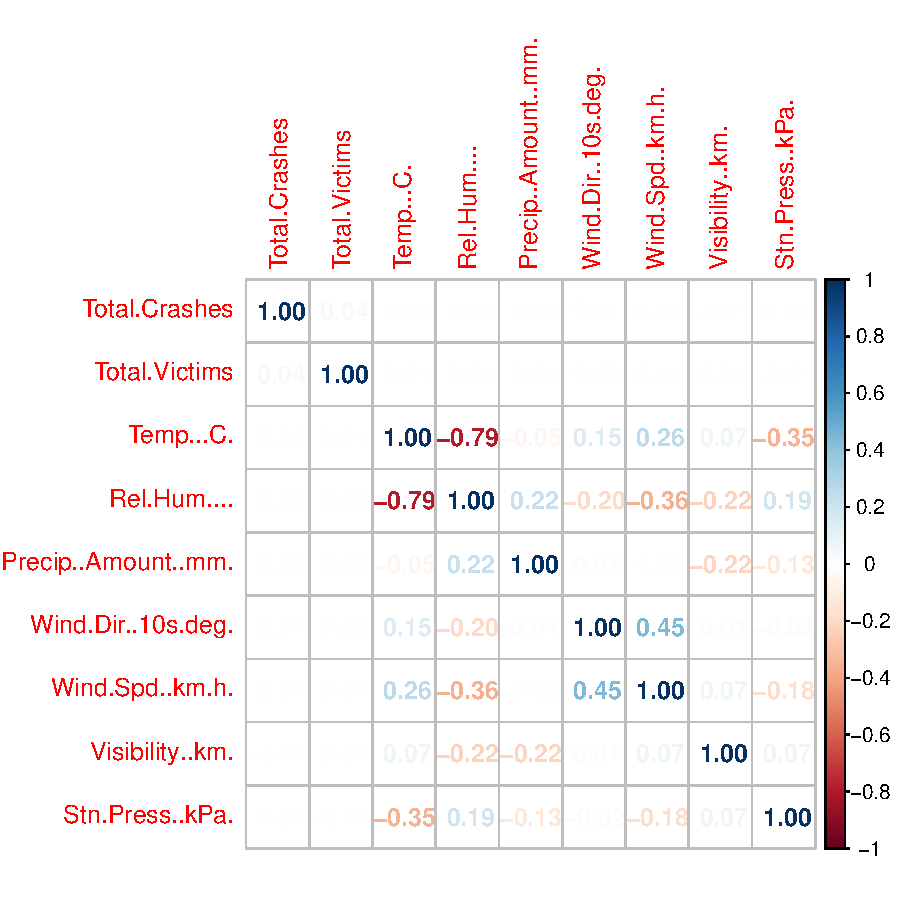
\includegraphics{variableinvestigation-ss}




\pagebreak
\section{Accidents over Time}

\subsection{Throughout the Day}



\subsection{Day of the Week} 

Distribution of accidents throughout the week:

\begin{Schunk}
\begin{Soutput}
   SUNDAY    MONDAY   TUESDAY WEDNESDAY  THURSDAY    FRIDAY  SATURDAY 
     5464      8024      8728      8790      9061      9316      6753 
\end{Soutput}
\end{Schunk}
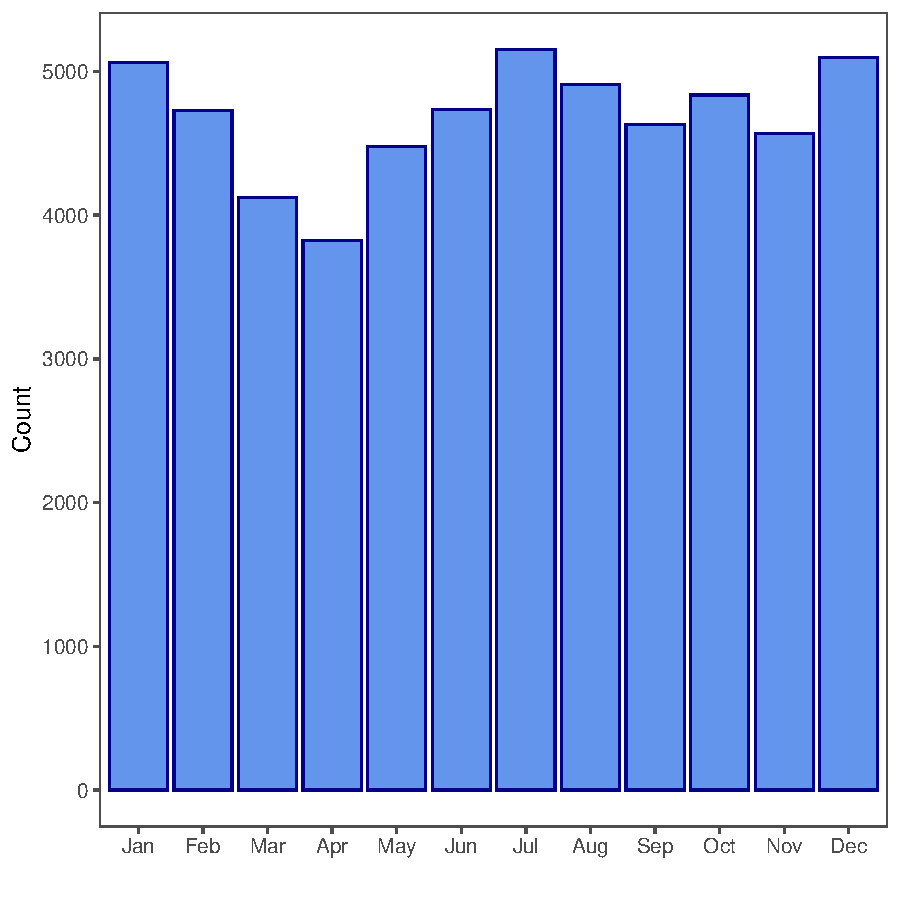
\includegraphics{variableinvestigation-004}


\pagebreak
\subsection{Month of the Year}

\begin{Schunk}
\begin{Soutput}
  JANUARY  FEBRUARY     MARCH     APRIL       MAY      JUNE      JULY    AUGUST 
     5063      4728      4120      3825      4475      4735      5152      4907 
SEPTEMBER   OCTOBER  NOVEMBER  DECEMBER 
     4632      4836      4568      5095 
\end{Soutput}
\end{Schunk}
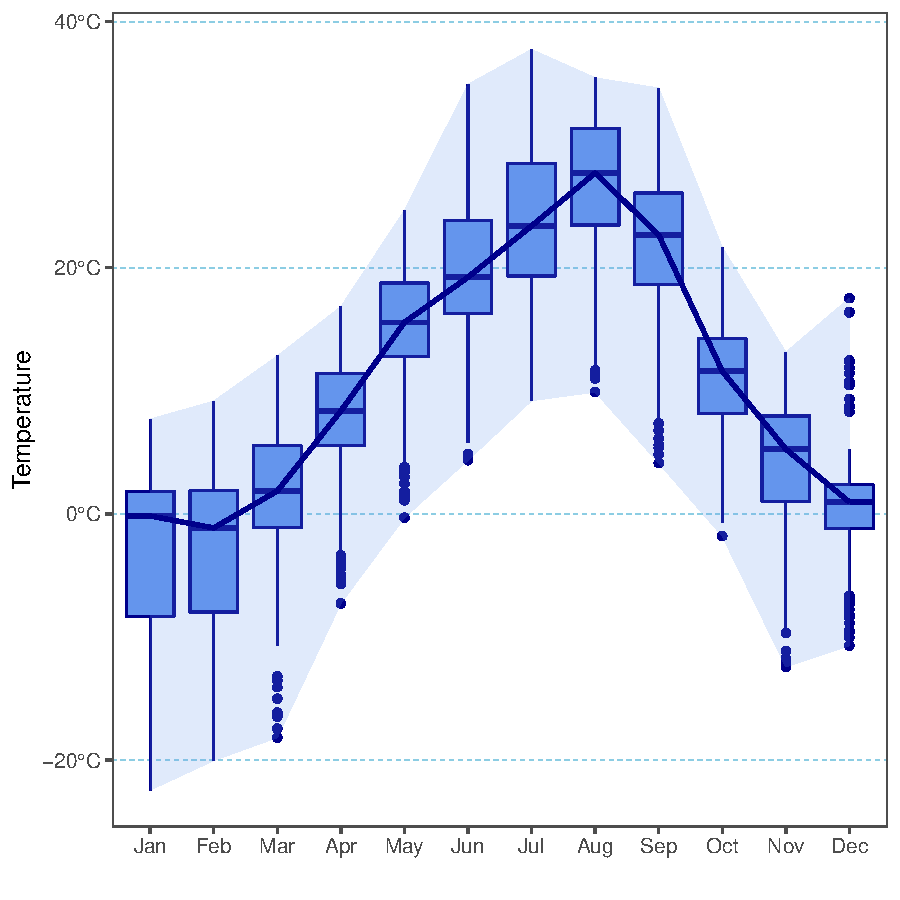
\includegraphics{variableinvestigation-005}


\pagebreak
\subsection{Over the Years}

\begin{Schunk}
\begin{Soutput}
 2017  2018  2019  2020  2021 
12734 12324 11148  9275 10655 
\end{Soutput}
\end{Schunk}
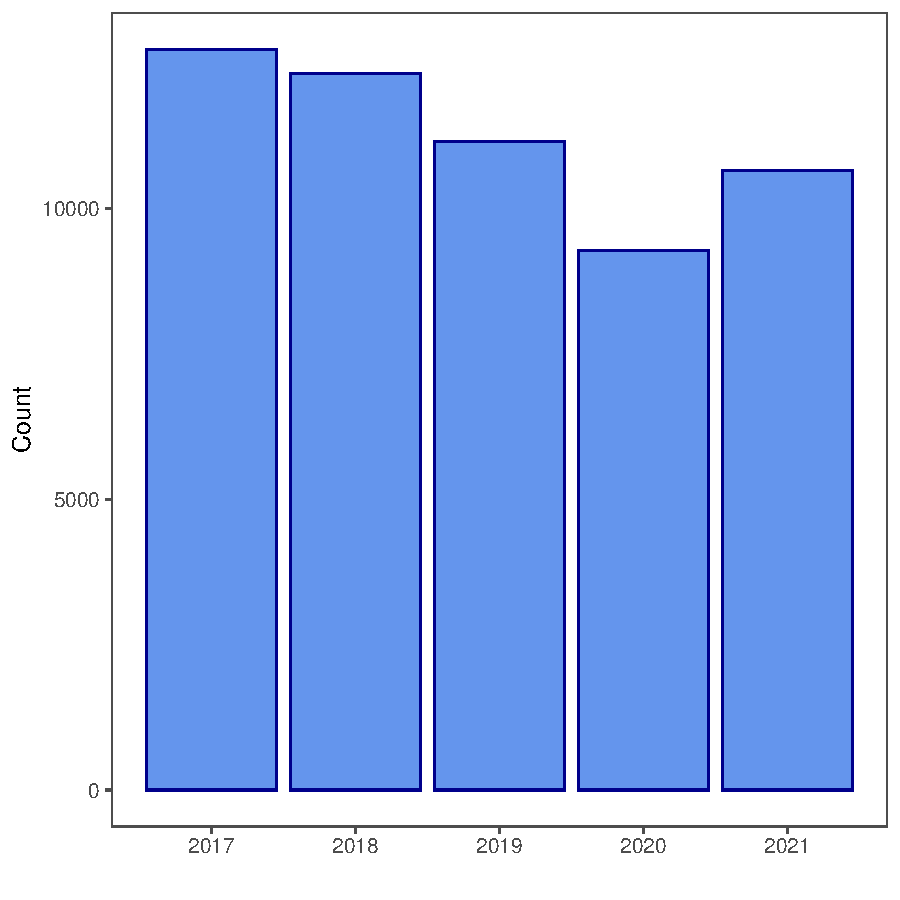
\includegraphics{variableinvestigation-006}





\pagebreak
\section{Distributions of Weather Variables}

\subsection{Temperature}


\begin{Schunk}
\begin{Soutput}
  Avg.temp. Avg.crash.temp.
1  8.511442        10.91872
\end{Soutput}
\end{Schunk}
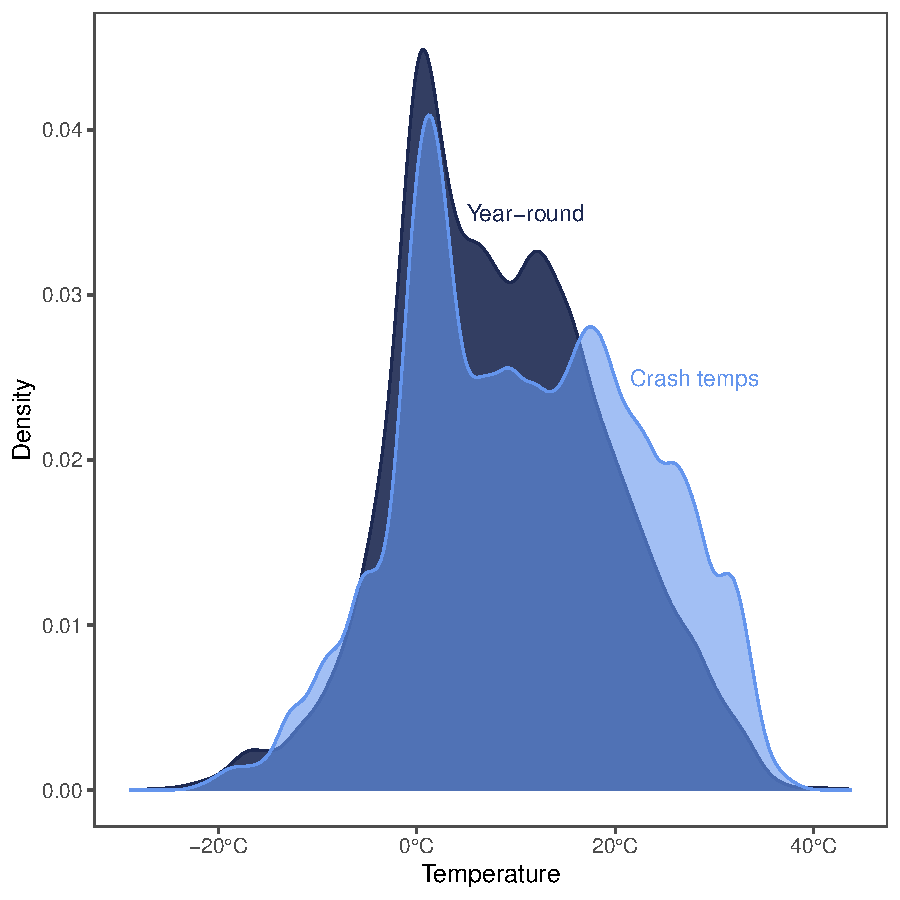
\includegraphics{variableinvestigation-008}



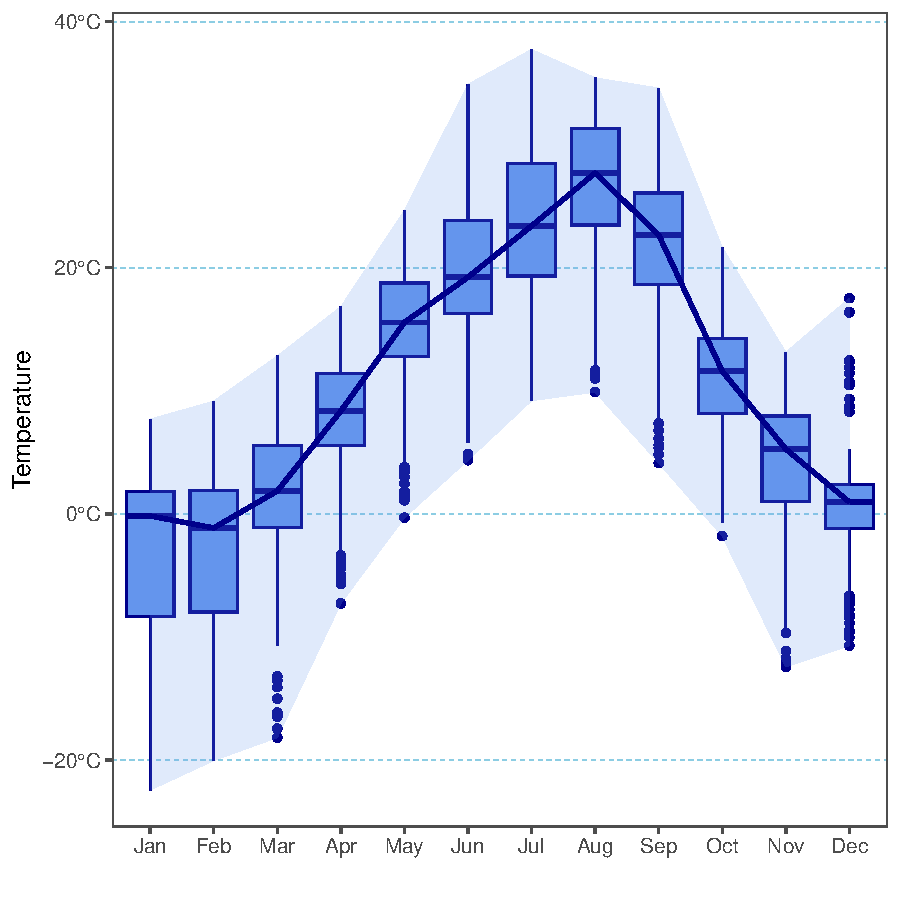
\includegraphics{variableinvestigation-009}



\pagebreak
\subsection{Relative Humidity}

\begin{Schunk}
\begin{Soutput}
  Avg.humidity Avg.crash.humidity
1     69.32555           60.50743
\end{Soutput}
\end{Schunk}
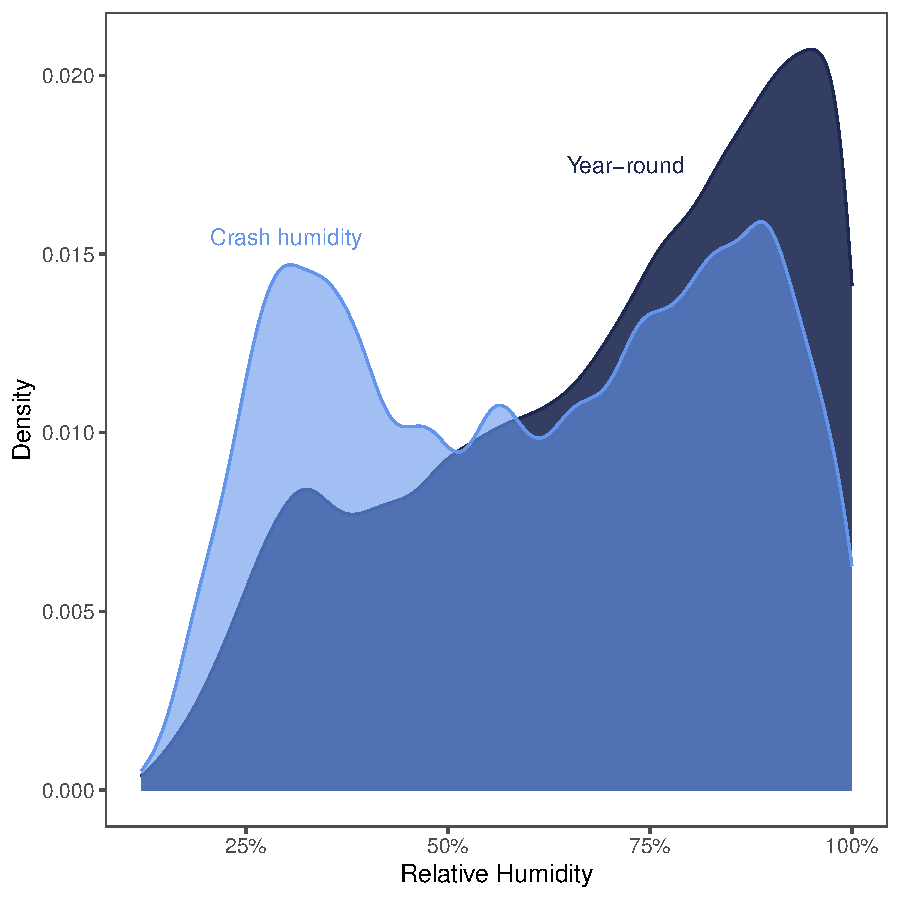
\includegraphics{variableinvestigation-010}

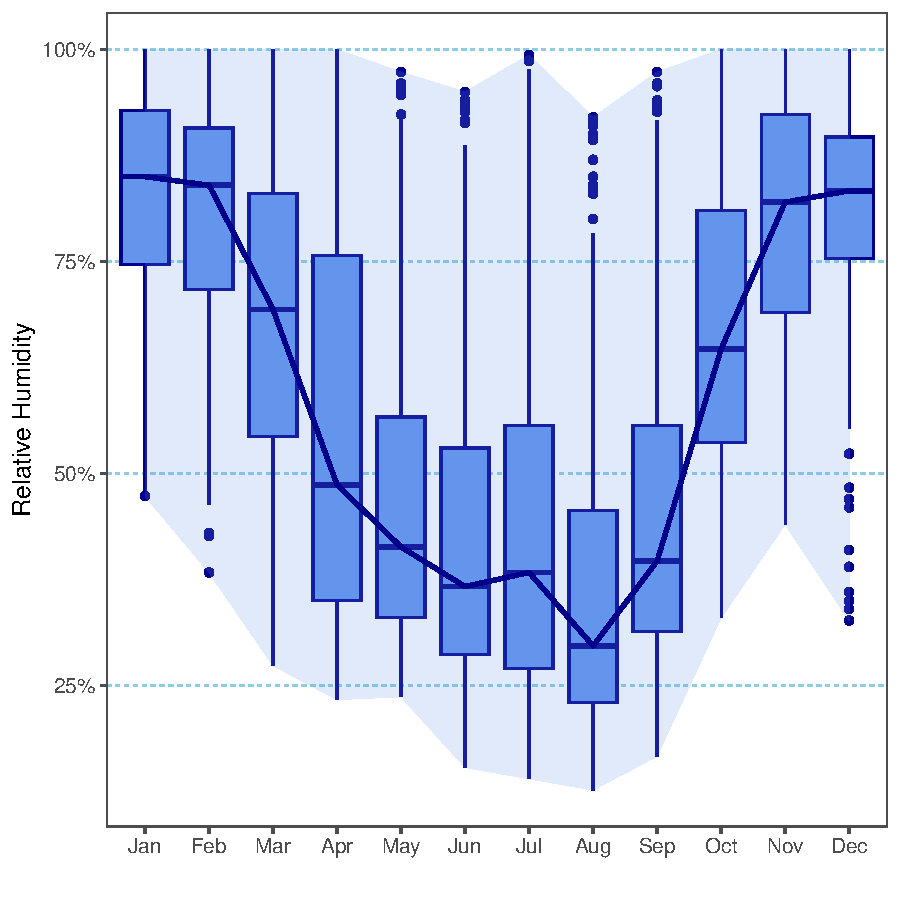
\includegraphics{variableinvestigation-011}



\pagebreak
\subsection{Precipitation}

\begin{Schunk}
\begin{Soutput}
  Avg.humidity Avg.crash.humidity
1   0.02998858         0.03110818
\end{Soutput}
\end{Schunk}




\pagebreak
\subsection{Wind Direction}





\pagebreak
\subsection{Visibility}





\pagebreak
\subsection{Air Pressure}









\section{Crash Subtypes}

\subsection{All Combined}

* nrow
* intersection flag
* months
* day of the week
* crash severity
* street name
* total victims
* avg temp, "Rel.Hum....", "Precip..Amount..mm.", 
"Wind.Dir..10s.deg.", "Wind.Spd..km.h.", "Visibility..km.", "Stn.Press..kPa."


\pagebreak
\subsection{Cyclist Crashes}








\pagebreak
\subsection{Animal Crashes}




\pagebreak
\subsection{Heavy Vehicle Crashes}




\pagebreak
\subsection{Motorcycle Crashes}




\pagebreak
\subsection{Parked Vehicle Crashes}





\pagebreak
\subsection{Pedestrian Crashes}











\pagebreak
\section{}






\end{document}
